% Control System Block Diagram
% Demonstrates: feedback loops, transfer functions, summing junctions, and blocks.
% Compile with: pdflatex main.tex

\documentclass[border=10pt]{standalone}
\usepackage{tikz}
\usetikzlibrary{arrows.meta, positioning, calc}

\begin{document}
\begin{tikzpicture}[
    >=Stealth,
    block/.style={
        draw, fill=blue!10, rectangle,
        minimum height=1.2cm, minimum width=2cm,
        font=\normalsize, text centered,
    },
    sum/.style={
        draw, fill=yellow!20, circle,
        minimum size=6mm, inner sep=0pt,
        font=\small,
    },
    input/.style={coordinate},
    output/.style={coordinate},
    thick,
    node distance=2cm,
]

% =============================================================================
% Diagram 1: Classic PID Feedback Loop
% =============================================================================
\begin{scope}[shift={(0,0)}]

    \node[font=\bfseries\large, above] at (6, 2.5) {PID Feedback Control System};

    % Input
    \node[input] (input) at (0, 0) {};
    \node[left] at (input) {$R(s)$};

    % Summing junction
    \node[sum] (sum) at (2, 0) {$\Sigma$};
    \node[below left, font=\scriptsize] at (sum.south west) {$+$};
    \node[above left, font=\scriptsize, text=red] at (sum.north west) {$-$};

    % Controller
    \node[block] (ctrl) at (5, 0) {$G_c(s)$};
    \node[font=\scriptsize, gray, above] at (ctrl.north) {Controller};

    % Plant
    \node[block] (plant) at (8.5, 0) {$G_p(s)$};
    \node[font=\scriptsize, gray, above] at (plant.north) {Plant};

    % Output
    \node[output] (output) at (11, 0) {};
    \node[right] at (output) {$Y(s)$};

    % Sensor / Feedback
    \node[block] (sensor) at (6.75, -2.5) {$H(s)$};
    \node[font=\scriptsize, gray, below] at (sensor.south) {Sensor};

    % Connections
    \draw[->] (input) -- (sum);
    \draw[->] (sum) -- node[above, font=\small] {$E(s)$} (ctrl);
    \draw[->] (ctrl) -- node[above, font=\small] {$U(s)$} (plant);
    \draw[->] (plant) -- (output);

    % Feedback path
    \draw[->] (9.75, 0) |- (sensor);
    \draw[->] (sensor) -| (sum);

    % Closed-loop transfer function annotation
    \node[font=\small, text=purple, align=center] at (6, -4.5) {%
        Closed-loop: $\dfrac{Y(s)}{R(s)} = \dfrac{G_c(s)\,G_p(s)}{1 + G_c(s)\,G_p(s)\,H(s)}$
    };

    % Feedback tap dot
    \filldraw (9.75, 0) circle (2pt);

\end{scope}

% =============================================================================
% Diagram 2: Cascade with Disturbance
% =============================================================================
\begin{scope}[shift={(0, -9)}]

    \node[font=\bfseries\large, above] at (7, 2.5) {Cascade System with Disturbance};

    % Input
    \node[input] (in) at (0, 0) {};
    \node[left] at (in) {$R(s)$};

    % Summing junction 1 (error)
    \node[sum] (s1) at (2, 0) {$\Sigma$};

    % Controller
    \node[block] (C) at (4.5, 0) {$C(s)$};

    % Summing junction 2 (disturbance)
    \node[sum] (s2) at (7, 0) {$\Sigma$};

    % Disturbance input
    \node[above] at (7, 1.5) {$D(s)$};
    \draw[->] (7, 1.5) -- (s2.north);
    \node[font=\scriptsize] at (7.3, 0.35) {$+$};
    \node[font=\scriptsize] at (6.65, -0.05) {$+$};

    % Plant
    \node[block] (P) at (9.5, 0) {$P(s)$};

    % Output
    \node[output] (out) at (12, 0) {};
    \node[right] at (out) {$Y(s)$};

    % Feedback
    \draw[->] (in) -- (s1);
    \draw[->] (s1) -- node[above, font=\small] {$E$} (C);
    \draw[->] (C) -- (s2);
    \draw[->] (s2) -- (P);
    \draw[->] (P) -- (out);

    % Unity feedback
    \draw[->] (11, 0) -- (11, -2) -| (s1);
    \filldraw (11, 0) circle (2pt);
    \node[font=\scriptsize, text=red] at (1.65, -0.35) {$-$};
    \node[font=\scriptsize] at (1.65, 0.35) {$+$};

\end{scope}

% =============================================================================
% Diagram 3: Signal Flow Simplification
% =============================================================================
\begin{scope}[shift={(0, -16)}]

    \node[font=\bfseries\large, above] at (5, 2) {Series-Parallel Reduction};

    % Series blocks
    \node[block] (G1) at (2, 0) {$G_1$};
    \node[block] (G2) at (5, 0) {$G_2$};
    \node[block] (G3) at (8, 0) {$G_3$};

    \draw[->] (0, 0) node[left] {$X$} -- (G1);
    \draw[->] (G1) -- (G2);
    \draw[->] (G2) -- (G3);
    \draw[->] (G3) -- (10, 0) node[right] {$Y$};

    % Equals sign
    \node[font=\Huge] at (11, 0) {$=$};

    % Equivalent single block
    \node[block, minimum width=3.5cm, fill=green!10] (Geq) at (14, 0) {$G_1 G_2 G_3$};
    \draw[->] (12, 0) node[left] {$X$} -- (Geq);
    \draw[->] (Geq) -- (16.5, 0) node[right] {$Y$};

\end{scope}

\end{tikzpicture}
\end{document}
